\section{The Ising model}\label{sec:ising_theory}

The Ising model consist of a lattice $\boldsymbol{\sigma}$ where each cite $\sigma \in \boldsymbol{\sigma}$, a point on the lattice, can have binary spin value $\sigma \in \{+1, -1\}$. The Hamiltonian function is given by

\begin{equation}
  H(\boldsymbol{\sigma}) =J\sum_{\langle i,j\rangle} \sigma^z_i\sigma^z_j + L \sum_j \sigma^x_j \; ,
  \label{eq:Ising_hamiltonian}
\end{equation}

where $i$ and $j$ are nearest neighbours on the lattice. The constant $J$ is the interaction, or coupling, strength while the constant $L$ is referred to and understood as the strength of a external magnetic field. The Hamiltonian function outputs the energy of a given configuration $\boldsymbol{\sigma}$.

For a one-dimensional Ising model we have a line of particles, here $N = 6$.

\begin{figure}[H]
  \begin{center}
    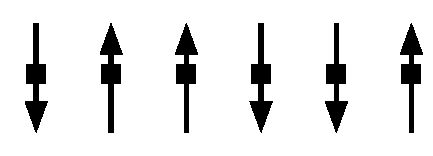
\includegraphics[width=0.5\textwidth]{Figures/Drawn/Ising/ising 1d}
  \end{center}
\end{figure}

and we would have interaction only on in one direction. An obvious problem occurs at the endpoints where the particles are missing a neighbour. There are two main solutions, to either place the boundary conditions $\sigma_{0} = \sigma_{2}$ together with $\sigma_{N+1} = \sigma_{N-1}$ or the condition $\sigma_{N+1} = \sigma_{1}$ and $\sigma_{-1} = \sigma_N$, where we will use the latter. This results in a continuous-like lattice:

\begin{figure}[H]
  \begin{center}
    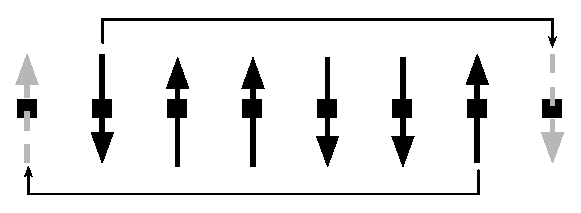
\includegraphics[width=0.5\textwidth]{Figures/Drawn/Ising/ising1dciclous}
  \end{center}
\end{figure}

To find the exact solution we want to diagonalize the Hamiltonian matrix, and from the Hamiltonian function we can interpret the spin operators $\sigma_i^x$ as the as a flip of the particle's spin at lattice point $i$. In vector form we can represent a lattice point by its spin:

\begin{equation}
  \downarrow \; = \ket{0} = \begin{bmatrix}
    1 \\ 0
    \end{bmatrix} \space\space\space\;\;\;\;\;\;\; \;\;\; \space\space\space \uparrow \; = \ket{1} = \begin{bmatrix}
  0 \\ 1
  \end{bmatrix} \; .
  \label{eq:ising_basis}
\end{equation}

A $N$-particle configuration we would represented as

$$\ket{\boldsymbol{\sigma}} = \ket{\sigma_1} \otimes \ket{\sigma_2} \otimes \dots \otimes \ket{\sigma_N} \; .$$

Changes to the configuration, or state, $\ket{\boldsymbol{\sigma}}$ through operators can be understood in matrix form. No change is done by the identity matrix $\mathbb{I}_{2^N}$, constructed by affecting each lattice point by $\mathbb{I}_2$:

$$\mathbb{I}_{2^N} = \mathbb{I}_{2, 1} \otimes \mathbb{I}_{2, 1} ... \otimes \mathbb{I}_{2, N} \; .$$

A spin flip by the external field part, with the Pauli matrices:

\[
\sigma_x =
\begin{pmatrix}0&1\\1&0\end{pmatrix}
\]
\[
\sigma_y =
\begin{pmatrix}0&-i\\i&0\end{pmatrix} 
\]
\[
\sigma_z =
\begin{pmatrix}1&0\\0&-1\end{pmatrix} \; ,
\] 

is then done by replacing the $\mathbb{I}_{2, i}$ with the spin matrix $\sigma_x$:

\begin{equation}
  \sigma_i^x = \mathbb{I}_{2, 1} \otimes \dots \otimes \sigma_{x, i} \otimes \dots \mathbb{I}_{2, N} \; .
  \label{eq:state_spin_z}
\end{equation}

The coupling interaction is interpreted as

\begin{equation}
  \sigma_i^z \sigma_{i+1}^z = \mathbb{I}_{2, 1} \otimes \dots \otimes \sigma_{z, i} \otimes \sigma_{z, i+1} \otimes \dots \otimes \mathbb{I}_{2, N} \; .
  \label{eq:coupling_spin}
\end{equation}

The Hamiltonian matrix can then be constructed by constructing and adding together each of the addend matrices. Further we have a grid of particles for the two-dimensional Ising model, here a $4\times 6$ grid:

\begin{figure}[H]
  \begin{center}
    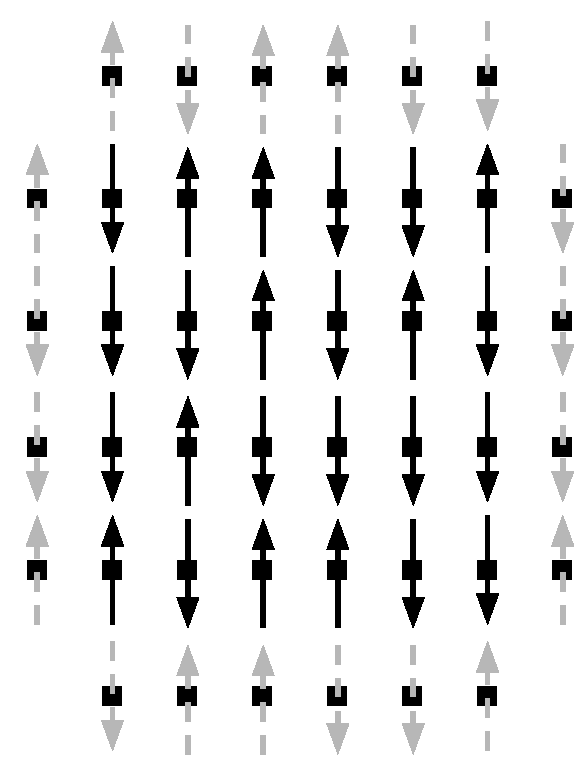
\includegraphics[width=0.5\textwidth]{Figures/Drawn/Ising/2dciclous}
  \end{center}
\end{figure}

The Hamiltonian function uses $\langle i, j\rangle$ to represent closest neighbouring lattice points, but for two dimensions specifically we can rewrite the Hamiltonian function as

\begin{equation}
  H_{2D}(\boldsymbol{\sigma}) =J\sum_{i = 1}^M\sum_{j = 1}^N \left (\sigma^z_{i, j}\sigma^z_{i, j + 1} + \sigma_{i, j}^z\sigma^z_{i+1, j} \right )+ L \sum_{i = 1}^M\sum_{j = 1}^N\sigma^z_{i, j} \; .
  \label{eq:2d_ising_ham_func}
\end{equation}

where $i$ is the $i$-th row and $j$ is the $j$-th particle in that row. The configuration is here represented in our basis by 

$$\ket{\boldsymbol{\sigma}}_{2D} = \ket{\sigma_{1, 1}} \otimes \ket{\sigma_{1, 2}} \otimes \dots \otimes \ket{\sigma_{1, N}} \otimes \ket{\sigma_{2, 1}} \otimes \dots \otimes \ket{\sigma_{M, N}}$$

Where we can then construct the Hamiltonian matrix the same way as explained for one dimension by following \ref{eq:2d_ising_ham_func} together with \ref{eq:state_spin_z} and \ref{eq:coupling_spin}.

\subsection{Solution by diagonalization}

If we take the transverse-field one-dimensional Ising model with two particles we have the Hamiltonian matrix constructed by:



$$ H =  L \left ( \sigma^x_1\otimes\mathbb{I} + \mathbb{I}\otimes\sigma_2^x \right ) + J \left (\sigma^z_1\otimes\sigma_2^z + \sigma_1^z\otimes\sigma_2^z \right ) \; ,$$

and we calculate the tensor products:

\begin{align*}
  \sigma^x\otimes\mathbb{I} &= \begin{bmatrix}
    0 & 1 & 0 & 0 \\
    1 & 0 & 0 & 0 \\
    0 & 0 & 0 & 1 \\
    0 & 0 & 1 & 0 \end{bmatrix} \\
    \mathbb{I}\otimes\sigma^x &= \begin{bmatrix}
    0 & 0 & 1 & 0 \\
    0 & 0 & 0 & 1 \\
    1 & 0 & 0 & 0 \\
    0 & 1 & 0 & 0\end{bmatrix} \\
      \sigma^z\otimes\sigma^z &= \begin{bmatrix}
    1 & 0 & 0 & 0 \\
    0 & -1 & 0 & 0 \\
    0 & 0 & -1 & 0 \\
    0 & 0 & 0 & 1\end{bmatrix}\; .
\end{align*}

We then get

\begin{equation}
  H_{J=1} =  \begin{bmatrix}
    J & L & L & 0 \\
    L & -J & 0 & L \\
    L & 0 & -J & L \\
  0 & L & L & J\end{bmatrix} \; ,
\end{equation}

and if with $L=-1$ and $J \in {-1, 1}$ we diagonalize and plot the eigenvalues:

\begin{figure}[H]
  \begin{center}
    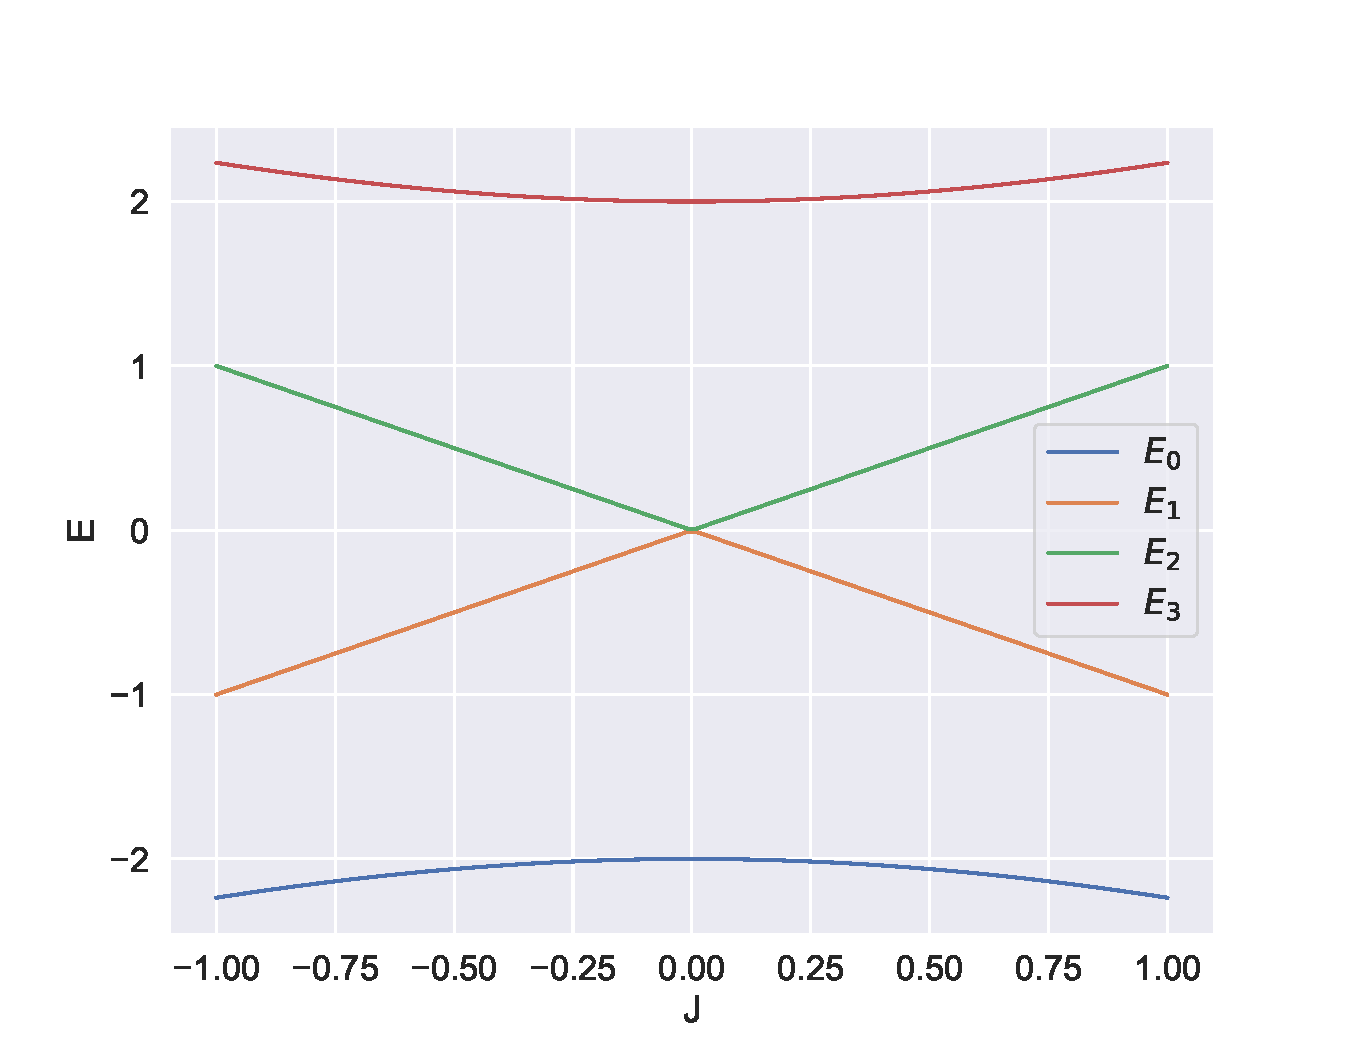
\includegraphics[width=0.95\textwidth]{Figures/Plots/Ising/ising_diag.pdf}
  \end{center}
  \caption{The energy derived from diagonalization of the $H_{J=1}$ Ising Hamiltonian with $L = 1$.}

\end{figure}

For a two-dimensional version we use four particles in a $2\times2$ grid, and with the same field strength we get:


\begin{figure}[H]
  \begin{center}
    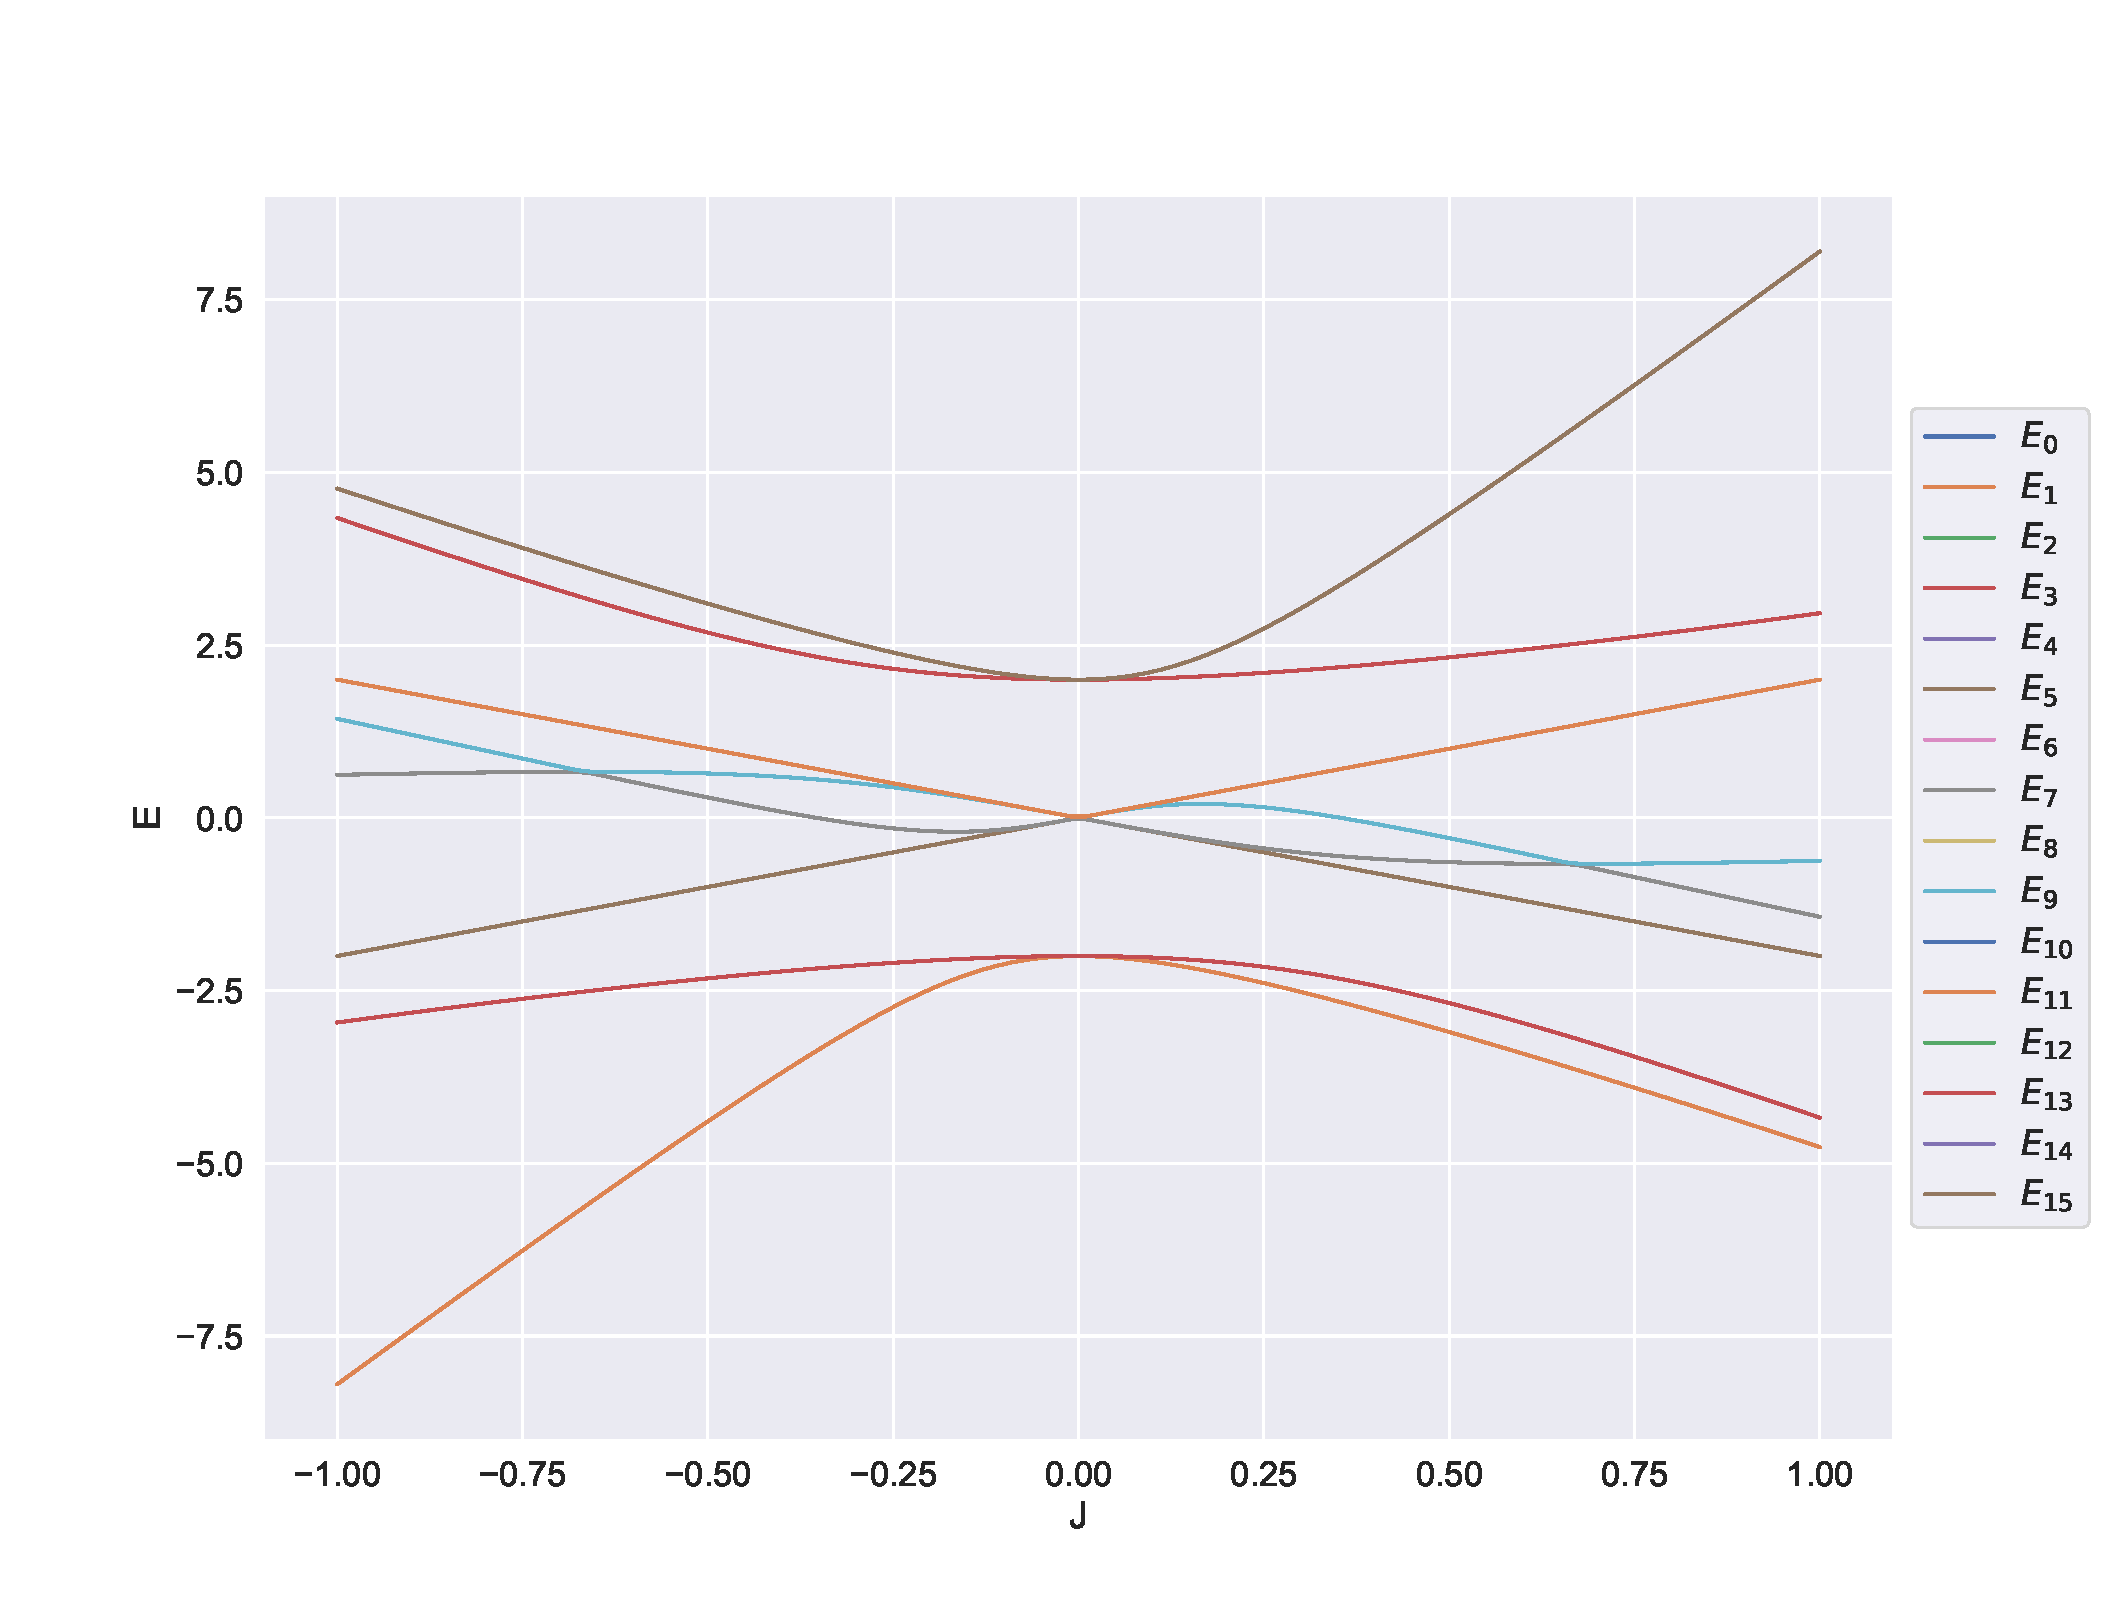
\includegraphics[width=0.95\textwidth]{Figures/Plots/Ising/ising_diag_42.pdf}
  \end{center}
  \caption{The energy derived from diagonalization of the $H_{J=2}$ two-dimensional Ising Hamiltonian with $L = 1$.}
\end{figure}

